\section{Partial Information}
\subsection{Redundancy Measure}
\begin{frame}{Redundancy Measure}
    Let $A_1, A_2, \ldots, A_k$ be nonempty and potentially overlapping
subsets of $R,$ which we call sources. We introduce $I_{\min}$ to measure the information that all sources provide about S.
\begin{definition}[Redundancy Measure]
\begin{equation}I_{\min }\left(S ;\left\{\mathbf{A}_{1}, \mathbf{A}_{2}, \ldots, \mathbf{A}_{k}\right\}\right)=\sum_{s} p(s) \min _{\mathbf{A}_{i}} I\left(S=s ; \mathbf{A}_{i}\right)\end{equation}
where the domain of $I_{\min}$ $\mathcal{A}(\mathbf{R})=\left\{\alpha \in \mathcal{P}_{1}\left(\mathcal{P}_{1}(\mathbf{R})\right): \forall \mathbf{A}_{i}, \mathbf{A}_{j} \in \alpha, \mathbf{A}_{i} \notin \mathbf{A}_{j}\right\}$
\end{definition}

\begin{block}{Properties of Redundancy Measure}
\begin{itemize}
    \item $I_{\min}$ is non-negative
    \item $I_{\min }$ is less than or equal to $I\left(S ; \mathbf{A}_{i}\right)$ for all $\mathbf{A}_{i}$ 's
    \item For a given source A, the amount of information redundant with $\mathbf{A}$ is maximal for $I_{\min }(S ;\{\mathbf{A}\})=I(S ; \mathbf{A}) .$
\end{itemize}
\end{block}
\end{frame}

\subsection{Relations between Redundancy Measures}
\begin{frame}{Relations between Redundancy Measures}
    Note that $I_{\min}$ can measure redundancy between collections of sources like $\left\{\left\{R_{1}\right\},\left\{R_{2}, R_{3}\right\}\right\}$ denoted as $\{1\}\{23\}$. Certain relations exists between measures.
    
    \begin{columns}
    \begin{column}{0.5\linewidth}
        \centering
        \begin{block}{Redundancy Order}
            We can define a partial order over the elements of $A(R)$ such that one is considered to precede another if and only if the latter provides any redundant information that the former provides. Formally,
            \begin{equation}\begin{aligned}&\forall \alpha, \beta \in \mathcal{A}(\mathbf{R}), \\
            &\alpha \preccurlyeq \beta \Leftrightarrow \forall \mathbf{B} \in \beta, \exists \mathbf{A} \in \alpha, \mathbf{A} \subseteq \mathbf{B}\end{aligned}\end{equation}
        \end{block}
    \end{column}
    \begin{column}{0.45\linewidth}
        \begin{figure}
            \centering
            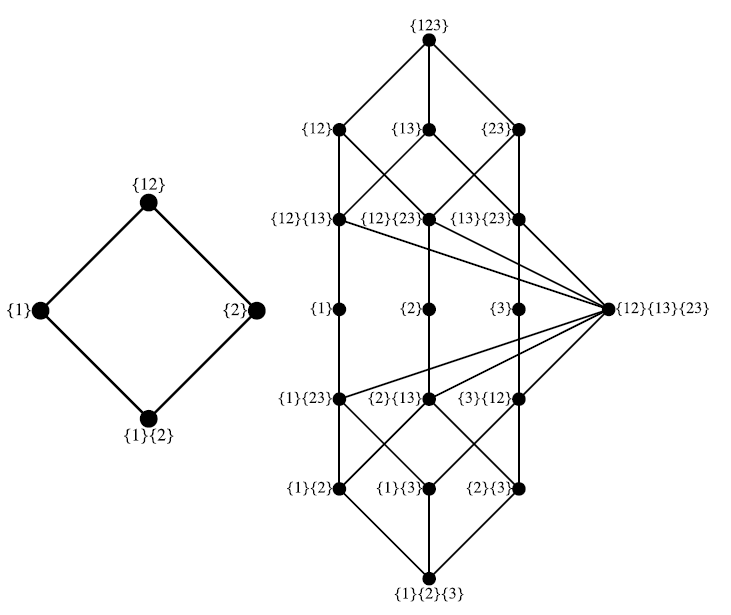
\includegraphics[width=0.8\linewidth]{img/lattic.png}
            \caption{Redundancy lattice for (A) 3 and (B) 4 variables.}
            \label{fig:lattice}
        \end{figure}
    \end{column}
    \end{columns}
\end{frame}

\subsection{Partial Information Decomposition}
\begin{frame}{Partial Information Decomposition}
    We would like to decompose redundancy measure into non-intersecting fragments. For a collection of sources $\alpha \in \mathcal{A}(\mathbf{R}),$ the PI-function denoted $\Pi_{\mathrm{R}},$ is defined implicitly by
    \begin{equation}
    I_{\min }(S ; \alpha)=\sum_{\beta \preccurlyeq \alpha} \Pi_{\mathrm{R}}(S ; \beta)
    \label{eee}
    \end{equation}
    
    \begin{columns}
    \begin{column}{0.5\linewidth}
    \begin{block}{Properties of Redundancy Measure}
    \begin{itemize}
        \item $\mathrm{II}_{\mathrm{R}}$ is non-negative
        \item $\mathrm{II}_{\mathrm{R}}$ can be calculated recursively.
        \item The relationship between these measures can be shown in a partial information (PI) diagram, which we will discuss later.
    \end{itemize}
    \end{block}
    \end{column}
    \begin{column}{0.45\linewidth}
        \begin{figure}
            \centering
            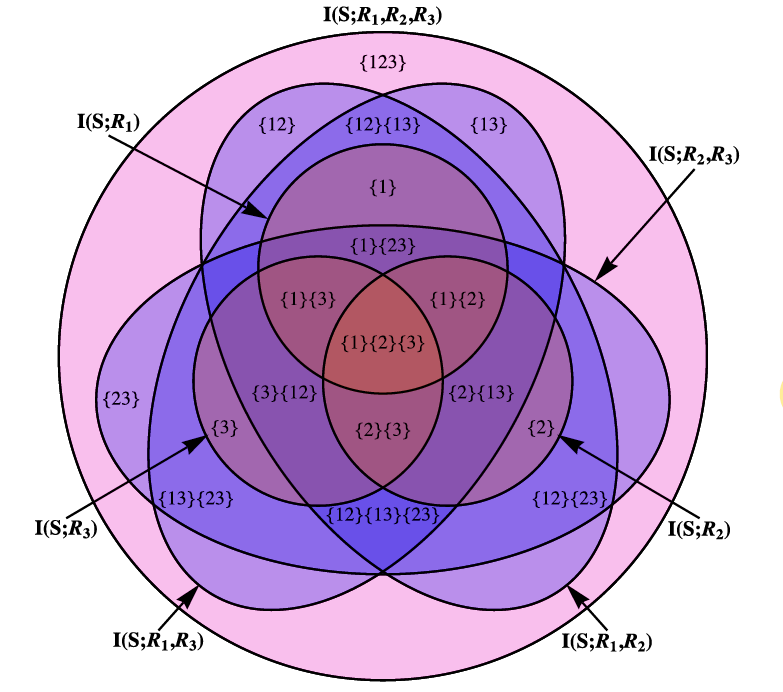
\includegraphics[width=0.8\linewidth]{img/partial4.png}
            \caption{PI diagram for 4 variables.}
            \label{fig:pi4}
        \end{figure}
    \end{column}
    \end{columns}
\end{frame}



